\documentclass[8pt,aspectratio=169]{beamer}
\usetheme{Madrid}
\usepackage{graphicx}
\usepackage{booktabs}
\usepackage{adjustbox}
\usepackage{multicol}
\usepackage{amsmath}
\usepackage{amssymb}
\usepackage{tikz}
\usepackage{hyperref}
\usepackage{algorithm}
\usepackage{algorithmic}
\usepackage{colortbl}
\usepackage{pgfplots}
\pgfplotsset{compat=1.18}

% TikZ libraries for comics, diagrams, stakeholder maps
\usetikzlibrary{arrows.meta,positioning,shapes.callouts,shapes.geometric,decorations.pathreplacing}

% Color definitions
\definecolor{mlblue}{RGB}{0,102,204}
\definecolor{mlpurple}{RGB}{51,51,178}
\definecolor{mllavender}{RGB}{173,173,224}
\definecolor{mllavender2}{RGB}{193,193,232}
\definecolor{mllavender3}{RGB}{204,204,235}
\definecolor{mllavender4}{RGB}{214,214,239}
\definecolor{mlorange}{RGB}{255, 127, 14}
\definecolor{mlgreen}{RGB}{44, 160, 44}
\definecolor{mlred}{RGB}{214, 39, 40}
\definecolor{mlgray}{RGB}{127, 127, 127}
\definecolor{lightgray}{RGB}{240, 240, 240}
\definecolor{midgray}{RGB}{180, 180, 180}

% NEW COLORS for mini-lecture
\definecolor{dfteal}{RGB}{0,128,128}
\definecolor{dfred}{RGB}{180,30,30}

% Backward compatibility
\colorlet{MLPurple}{mlpurple}
\colorlet{MLBlue}{mlblue}
\colorlet{MLOrange}{mlorange}
\colorlet{MLGreen}{mlgreen}
\colorlet{MLRed}{mlred}
\colorlet{MLLavender}{mllavender}
\colorlet{MLGray}{mlgray}

% Theme colors (exact Madrid settings)
\setbeamercolor{palette primary}{bg=mllavender3,fg=mlpurple}
\setbeamercolor{palette secondary}{bg=mllavender2,fg=mlpurple}
\setbeamercolor{palette tertiary}{bg=mllavender,fg=white}
\setbeamercolor{palette quaternary}{bg=mlpurple,fg=white}
\setbeamercolor{structure}{fg=mlpurple}
\setbeamercolor{section in toc}{fg=mlpurple}
\setbeamercolor{subsection in toc}{fg=mlblue}
\setbeamercolor{title}{fg=mlpurple}
\setbeamercolor{frametitle}{fg=mlpurple,bg=mllavender3}
\setbeamercolor{block title}{bg=mllavender2,fg=mlpurple}
\setbeamercolor{block body}{bg=mllavender4,fg=black}
\setbeamertemplate{navigation symbols}{}
\setbeamertemplate{itemize items}[circle]
\setbeamertemplate{enumerate items}[default]
\setbeamersize{text margin left=5mm,text margin right=5mm}

% Footer
\setbeamertemplate{footline}{
  \leavevmode%
  \hbox{%
    \begin{beamercolorbox}[wd=.333333\paperwidth,ht=2.25ex,dp=1ex,center]{author in head/foot}%
      \usebeamerfont{author in head/foot}Methods and Algorithms
    \end{beamercolorbox}%
    \begin{beamercolorbox}[wd=.333333\paperwidth,ht=2.25ex,dp=1ex,center]{title in head/foot}%
      \usebeamerfont{title in head/foot}MSc Data Science
    \end{beamercolorbox}%
    \begin{beamercolorbox}[wd=.333333\paperwidth,ht=2.25ex,dp=1ex,right]{date in head/foot}%
      \usebeamerfont{date in head/foot}\insertframenumber{} / \inserttotalframenumber\hspace*{2ex}
    \end{beamercolorbox}}%
  \vskip0pt%
}

\newcommand{\bottomnote}[1]{%
\vfill
\vspace{-2mm}
\textcolor{mllavender2}{\rule{\textwidth}{0.4pt}}
\vspace{1mm}
\footnotesize
\textbf{#1}
}

\newenvironment{compactlist}{%
  \begin{itemize}%
    \setlength{\itemsep}{2pt}%
    \setlength{\parskip}{0pt}%
    \setlength{\parsep}{0pt}%
}{%
  \end{itemize}%
}

\newcommand{\highlight}[1]{\textcolor{mlorange}{\textbf{#1}}}
\newcommand{\mathbold}[1]{\boldsymbol{#1}}

\title[Linear Regression Mini-Lecture]{Linear Regression}
\subtitle{Mini-Lecture: From Scatter Plots to Predictions}
\author{Methods \& Algorithms}
\date{MSc Data Science -- Spring 2026}

\begin{document}

%% ================================================================
%% SLIDE 1: Title Page
%% ================================================================
\begin{frame}[plain]
\titlepage
\end{frame}

%% ================================================================
%% SLIDE 2: Opening XKCD
%% ================================================================
\begin{frame}[t]{The Eternal Temptation of Fitting a Line}
\begin{center}
\includegraphics[width=0.6\textwidth]{images/1725_linear_regression.png}
\end{center}

\bottomnote{XKCD \#1725 by Randall Munroe (CC BY-NC 2.5)}
\end{frame}

%% ================================================================
%% SLIDE 3: The Problem
%% ================================================================
\begin{frame}[t]{The Problem: Predicting Outcomes from Data}
\begin{columns}[T]
\column{0.55\textwidth}
\small
\textbf{From Scatter Plot to Prediction}
\begin{compactlist}
\item A bank wants to predict house prices from square footage, location, and age
\item Each data point is a past transaction -- features on the x-axis, price on the y-axis
\item Can we draw a line through the cloud that generalizes to new houses?
\end{compactlist}

\begin{block}{Key Question}
\scriptsize How do we find the ``best'' line, and what does ``best'' even mean?
\end{block}

\column{0.42\textwidth}
\vspace{2mm}
\includegraphics[width=0.55\textwidth]{01_simple_regression/chart.pdf}
\end{columns}

\bottomnote{Linear regression is the foundation of predictive modeling -- nearly every ML method builds on or departs from it}
\end{frame}

%% ================================================================
%% SLIDE 4: The Idea
%% ================================================================
\begin{frame}[t]{The Idea: Fit a Line That Minimizes Error}
\begin{columns}[T]
\column{0.55\textwidth}
\small
\textbf{The Linear Model}
\begin{compactlist}
\item Model: $\hat{y} = \beta_0 + \beta_1 x_1 + \beta_2 x_2 + \cdots + \beta_p x_p$
\item $\beta_0$ is the intercept (baseline prediction)
\item Each $\beta_j$ captures the effect of feature $x_j$ on the outcome
\item ``Best'' means minimizing the total distance between predictions and actual values
\end{compactlist}

\column{0.42\textwidth}
\vspace{4mm}
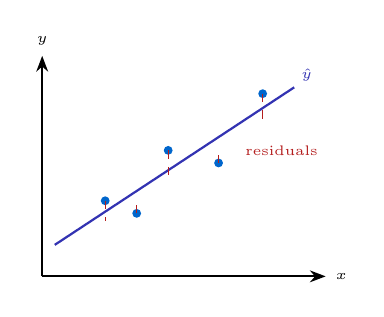
\begin{tikzpicture}[scale=0.8]
% Axes
\draw[-{Stealth[length=2mm]}, thick] (0,0) -- (4.5,0) node[right, font=\tiny] {$x$};
\draw[-{Stealth[length=2mm]}, thick] (0,0) -- (0,3.5) node[above, font=\tiny] {$y$};
% Best fit line
\draw[mlpurple, thick] (0.2,0.5) -- (4.0,3.0);
% Data points with residual lines
\fill[mlblue] (1.0,1.2) circle (0.07); \draw[dfred, dashed] (1.0,1.2) -- (1.0,0.88);
\fill[mlblue] (1.5,1.0) circle (0.07); \draw[dfred, dashed] (1.5,1.0) -- (1.5,1.2);
\fill[mlblue] (2.0,2.0) circle (0.07); \draw[dfred, dashed] (2.0,2.0) -- (2.0,1.52);
\fill[mlblue] (2.8,1.8) circle (0.07); \draw[dfred, dashed] (2.8,1.8) -- (2.8,2.03);
\fill[mlblue] (3.5,2.9) circle (0.07); \draw[dfred, dashed] (3.5,2.9) -- (3.5,2.48);
% Labels
\node[font=\tiny, dfred] at (3.8,2.0) {residuals};
\node[font=\tiny, mlpurple] at (4.2,3.2) {$\hat{y}$};
\end{tikzpicture}
\end{columns}

\bottomnote{The residuals (red dashes) are the errors we want to make as small as possible}
\end{frame}

%% ================================================================
%% SLIDE 5: OLS
%% ================================================================
\begin{frame}[t]{Ordinary Least Squares: The Closed-Form Solution}
\begin{columns}[T]
\column{0.55\textwidth}
\small
\textbf{Minimize Squared Residuals}
\begin{compactlist}
\item Loss function: $L(\beta) = \sum_{i=1}^{n}(y_i - \mathbf{x}_i^T\beta)^2$
\item Take derivative, set to zero, solve
\item Closed-form solution:
\end{compactlist}

\vspace{2mm}
\[\hat{\beta} = (X^TX)^{-1}X^Ty\]

\vspace{1mm}
\scriptsize This gives the unique global minimum -- no iteration needed.

\begin{block}{Insight}
\scriptsize OLS is fast and exact, but requires $X^TX$ to be invertible. When features are correlated, this breaks down -- motivating regularization.
\end{block}

\column{0.42\textwidth}
\vspace{4mm}
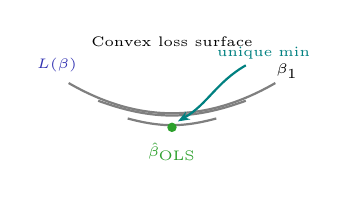
\begin{tikzpicture}[scale=0.75]
% Loss surface (bowl shape)
\draw[mlgray, thick] (0.5,2.5) to[out=-30,in=210] (4.0,2.5);
\draw[mlgray, thick] (1.0,2.2) to[out=-20,in=200] (3.5,2.2);
\draw[mlgray, thick] (1.5,1.9) to[out=-15,in=195] (3.0,1.9);
% Minimum point
\fill[mlgreen] (2.25,1.75) circle (0.08);
\node[font=\tiny, mlgreen, below] at (2.25,1.65) {$\hat{\beta}_{\text{OLS}}$};
% Axes labels
\node[font=\tiny, mlpurple] at (0.3,2.8) {$L(\beta)$};
\node[font=\tiny] at (4.2,2.7) {$\beta_1$};
\node[font=\tiny] at (2.25,3.2) {Convex loss surface};
% Arrow to minimum
\draw[-{Stealth[length=1.5mm]}, dfteal, thick] (3.5,2.8) to[out=210,in=30] (2.35,1.85);
\node[font=\tiny, dfteal] at (3.8,3.0) {unique min};
\end{tikzpicture}
\end{columns}

\bottomnote{OLS assumes: linearity, independence, homoscedasticity, normality of residuals (LINE assumptions)}
\end{frame}

%% ================================================================
%% SLIDE 6: Model Quality
%% ================================================================
\begin{frame}[t]{How Good Is Our Model?}
\begin{columns}[T]
\column{0.55\textwidth}
\small
\textbf{Evaluating Fit Quality}
\begin{compactlist}
\item \highlight{$R^2$}: fraction of variance explained, $R^2 = 1 - \frac{\text{SS}_{\text{res}}}{\text{SS}_{\text{tot}}}$
\item $R^2 = 1$ means perfect fit; $R^2 = 0$ means no better than the mean
\item \highlight{Residual plots} reveal model violations: patterns mean the model is wrong
\end{compactlist}

\begin{block}{Insight}
\scriptsize A high $R^2$ does not mean the model is correct -- always check residual plots for non-linearity and heteroscedasticity.
\end{block}

\column{0.42\textwidth}
\vspace{2mm}
\includegraphics[width=0.55\textwidth]{03_residual_plots/chart.pdf}
\end{columns}

\bottomnote{Residuals should look like random noise. Any pattern signals a missing variable or wrong functional form.}
\end{frame}

%% ================================================================
%% SLIDE 7: Gradient Descent
%% ================================================================
\begin{frame}[t]{Gradient Descent: The Iterative Alternative}
\begin{columns}[T]
\column{0.55\textwidth}
\small
\textbf{When OLS Is Too Expensive}
\begin{compactlist}
\item For millions of rows, inverting $X^TX$ is slow
\item \highlight{Gradient descent}: update weights iteratively
\[\beta_{t+1} = \beta_t - \alpha \nabla L(\beta_t)\]
\item $\alpha$ is the \highlight{learning rate} -- too large overshoots, too small is slow
\item Stochastic GD uses mini-batches for speed
\end{compactlist}

\begin{block}{Insight}
\scriptsize Gradient descent scales to any dataset size and generalizes to non-linear models -- it is the engine behind deep learning.
\end{block}

\column{0.42\textwidth}
\vspace{2mm}
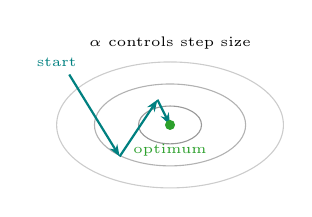
\begin{tikzpicture}[scale=0.8]
% Contour ellipses
\draw[mlgray!40] (2.0,2.0) ellipse (1.8 and 1.0);
\draw[mlgray!60] (2.0,2.0) ellipse (1.2 and 0.65);
\draw[mlgray!80] (2.0,2.0) ellipse (0.5 and 0.3);
% GD path
\draw[-{Stealth[length=1.5mm]}, dfteal, thick] (0.4,2.8) -- (1.2,1.5);
\draw[-{Stealth[length=1.5mm]}, dfteal, thick] (1.2,1.5) -- (1.8,2.4);
\draw[-{Stealth[length=1.5mm]}, dfteal, thick] (1.8,2.4) -- (2.0,2.0);
\fill[mlgreen] (2.0,2.0) circle (0.08);
% Labels
\node[font=\tiny, dfteal] at (0.2,3.0) {start};
\node[font=\tiny, mlgreen, below] at (2.0,1.85) {optimum};
\node[font=\tiny] at (2.0,3.3) {$\alpha$ controls step size};
\end{tikzpicture}
\end{columns}

\bottomnote{OLS: exact but $O(p^3)$. Gradient descent: approximate but $O(np)$ per step -- choose based on data size.}
\end{frame}

%% ================================================================
%% SLIDE 8: Regularization
%% ================================================================
\begin{frame}[t]{Regularization: Preventing Overfitting}
\begin{columns}[T]
\column{0.55\textwidth}
\small
\textbf{Ridge (L2) vs Lasso (L1)}
\begin{compactlist}
\item \highlight{Ridge}: adds $\lambda\sum\beta_j^2$ to loss -- shrinks coefficients toward zero
\item \highlight{Lasso}: adds $\lambda\sum|\beta_j|$ to loss -- drives some coefficients exactly to zero (feature selection)
\item $\lambda$ controls the trade-off: more regularization = simpler model
\end{compactlist}

\vspace{1mm}
\scriptsize Elastic Net combines both: $\lambda_1\sum|\beta_j| + \lambda_2\sum\beta_j^2$

\begin{block}{Insight}
\scriptsize Use Ridge when all features matter; use Lasso when you suspect many features are irrelevant. Cross-validate $\lambda$.
\end{block}

\column{0.42\textwidth}
\vspace{2mm}
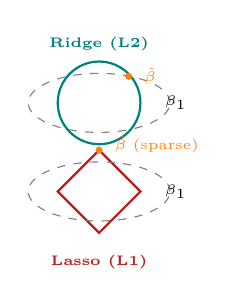
\begin{tikzpicture}[scale=0.75]
% L2 constraint (circle)
\draw[dfteal, thick] (1.2,3.2) circle (0.7);
\node[font=\tiny, dfteal] at (1.2,4.2) {\textbf{Ridge (L2)}};
% Contour ellipse touching circle
\draw[mlgray, dashed] (1.2,3.2) ellipse (1.2 and 0.5);
\fill[mlorange] (1.7,3.65) circle (0.06);
\node[font=\tiny, mlorange, right] at (1.8,3.65) {$\hat{\beta}$};
% L1 constraint (diamond)
\draw[dfred, thick] (1.2,1.0) -- (1.9,1.7) -- (1.2,2.4) -- (0.5,1.7) -- cycle;
\node[font=\tiny, dfred] at (1.2,0.5) {\textbf{Lasso (L1)}};
% Contour ellipse touching diamond corner
\draw[mlgray, dashed] (1.2,1.7) ellipse (1.2 and 0.5);
\fill[mlorange] (1.2,2.4) circle (0.06);
\node[font=\tiny, mlorange, right] at (1.3,2.5) {$\hat{\beta}$ (sparse)};
% Axes
\node[font=\tiny] at (2.5,3.2) {$\beta_1$};
\node[font=\tiny] at (2.5,1.7) {$\beta_1$};
\end{tikzpicture}
\end{columns}

\bottomnote{Lasso's diamond constraint has corners on the axes -- this is why it produces exact zeros (sparsity)}
\end{frame}

%% ================================================================
%% SLIDE 9: Finance Application
%% ================================================================
\begin{frame}[t]{Finance Application: CAPM and Factor Models}
\begin{columns}[T]
\column{0.55\textwidth}
\small
\textbf{Linear Regression in Finance}
\begin{compactlist}
\item \highlight{CAPM}: $R_i = \alpha + \beta R_m + \epsilon$
\item $\beta$ measures sensitivity to market risk; $\alpha$ is excess return
\item \highlight{Factor models}: extend to multiple risk factors (Fama-French 3-factor, Carhart 4-factor)
\item Portfolio risk decomposition via regression coefficients
\end{compactlist}

\begin{block}{Insight}
\scriptsize Every hedge fund's risk report is built on linear regression. The $\beta$ to market, size, value, and momentum factors determines portfolio exposure.
\end{block}

\column{0.42\textwidth}
\vspace{2mm}
\footnotesize
\fcolorbox{mlpurple}{mllavender4}{\parbox{0.85\columnwidth}{%
\textbf{Fama-French 3-Factor Model:}

\vspace{2mm}
$R_i - R_f = \alpha + \beta_1(R_m - R_f)$

$\quad + \beta_2 \cdot \text{SMB} + \beta_3 \cdot \text{HML} + \epsilon$

\vspace{2mm}
\textbf{SMB}: Small Minus Big (size)\\
\textbf{HML}: High Minus Low (value)
}}
\end{columns}

\bottomnote{CAPM won the Nobel Prize (Sharpe, 1990). Linear regression is the language of asset pricing.}
\end{frame}

%% ================================================================
%% SLIDE 10: Summary
%% ================================================================
\begin{frame}[t]{Summary: Linear Regression in 4 Takeaways}
\begin{columns}[T]
\column{0.95\textwidth}
\small
\begin{enumerate}
\setlength{\itemsep}{6pt}
\item \highlight{The model}: $\hat{y} = X\beta$ -- a linear combination of features, solved exactly via OLS or iteratively via gradient descent
\item \highlight{Evaluation}: $R^2$ measures fit quality, but always check residual plots -- a good $R^2$ can hide a bad model
\item \highlight{Regularization}: Ridge (L2) shrinks all coefficients; Lasso (L1) sets irrelevant ones to zero. Cross-validate $\lambda$.
\item \highlight{Finance}: CAPM and factor models are linear regressions -- $\beta$ is the language of risk
\end{enumerate}

\vspace{4mm}
\begin{block}{Next Steps}
\scriptsize Explore the deep dive slides for matrix derivations, statistical inference, and multicollinearity diagnostics. Try the Jupyter notebook to fit regressions on real housing data.
\end{block}
\end{columns}

\bottomnote{Linear regression is the starting point for all of machine learning -- master it before moving on}
\end{frame}

\end{document}
